% This file was created by matlab2tikz.
%
%The latest updates can be retrieved from
%  http://www.mathworks.com/matlabcentral/fileexchange/22022-matlab2tikz-matlab2tikz
%where you can also make suggestions and rate matlab2tikz.
%
\definecolor{mycolor1}{rgb}{0.00000,0.44700,0.74100}%
\definecolor{mycolor2}{rgb}{0.92900,0.69400,0.12500}%
\definecolor{mycolor3}{rgb}{0.46600,0.67400,0.18800}%
\definecolor{mycolor4}{rgb}{0.63500,0.07800,0.18400}%
\definecolor{mycolor5}{rgb}{0.85000,0.32500,0.09800}%
%
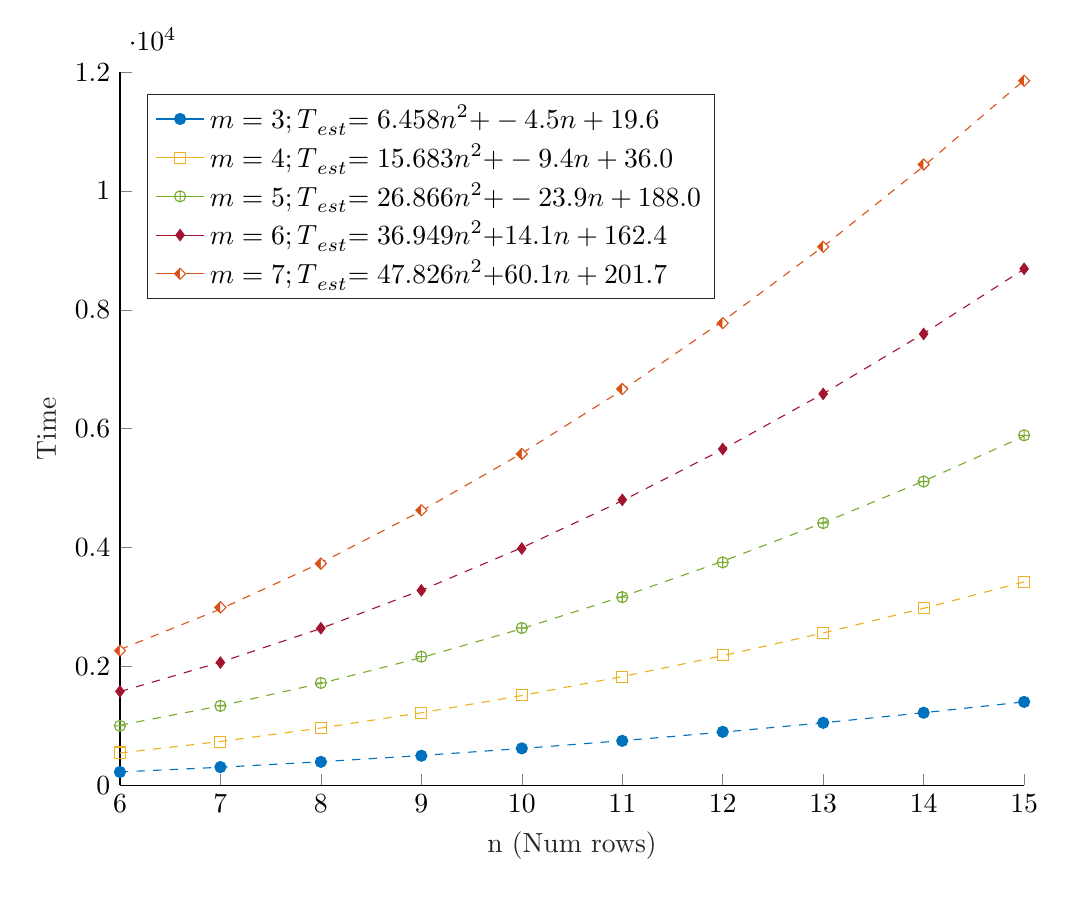
\begin{tikzpicture}

\begin{axis}[%
width=4.521in,
height=3.566in,
at={(0.758in,0.481in)},
scale only axis,
xmin=6,
xmax=15,
xlabel style={font=\color{white!15!black}},
xlabel={n (Num rows)},
ymin=0,
ymax=12000,
ylabel style={font=\color{white!15!black}},
ylabel={Time},
axis background/.style={fill=white},
title style={font=\bfseries},
% title={$\text{Average ticks until solution as a function of n. On n }\times\text{ m grid. (k = 1)}$},
axis x line*=bottom,
axis y line*=left,
legend style={at={(0.03,0.97)}, anchor=north west, legend cell align=left, align=left, draw=white!15!black}
]
\addplot [color=mycolor1, draw=none, mark=*, mark options={solid, mycolor1}]
  table[row sep=crcr]{%
6	224.722\\
7	307.388\\
8	395.078\\
9	498.208\\
10	621.888\\
11	748.38\\
12	900.358\\
13	1052.224\\
14	1221.764\\
15	1403.72\\
};
\addlegendentry{$\text{m = 3; T}_{\text{est}}\text{ =  6.458n}^\text{2}\text{ +  -4.5n +  19.6}$}

\addplot [color=mycolor1, dashed, forget plot]
  table[row sep=crcr]{%
6	224.950836363641\\
7	304.380327272729\\
8	396.725606060605\\
9	501.98667272727\\
10	620.163527272724\\
11	751.256169696966\\
12	895.264599999997\\
13	1052.18881818182\\
14	1222.02882424243\\
15	1404.78461818182\\
};
\addplot [color=mycolor2, draw=none, mark=square, mark options={solid, mycolor2}]
  table[row sep=crcr]{%
6	551.422\\
7	731.714\\
8	958.91\\
9	1221.578\\
10	1517.23\\
11	1819.998\\
12	2192.036\\
13	2561.248\\
14	2982.672\\
15	3418.84\\
};
\addlegendentry{$\text{m = 4; T}_{\text{est}}\text{ = 15.683n}^\text{2}\text{ +  -9.4n +  36.0}$}

\addplot [color=mycolor2, dashed, forget plot]
  table[row sep=crcr]{%
6	544.058072727263\\
7	738.525587878784\\
8	964.360012121212\\
9	1221.56134545455\\
10	1510.12958787879\\
11	1830.06473939394\\
12	2181.3668\\
13	2564.03576969697\\
14	2978.07164848485\\
15	3423.47443636363\\
};
\addplot [color=mycolor3, draw=none, mark=oplus, mark options={solid, mycolor3}]
  table[row sep=crcr]{%
6	1000.742\\
7	1336.826\\
8	1723.12\\
9	2165.81\\
10	2647.382\\
11	3166.968\\
12	3750.928\\
13	4413.322\\
14	5111.72\\
15	5889.168\\
};
\addlegendentry{$\text{m = 5; T}_{\text{est}}\text{ = 26.866n}^\text{2}\text{ + -23.9n + 188.0}$}

\addplot [color=mycolor3, dashed, forget plot]
  table[row sep=crcr]{%
6	1011.72909090911\\
7	1337.08401212122\\
8	1716.16996363636\\
9	2148.98694545453\\
10	2635.53495757574\\
11	3175.81399999998\\
12	3769.82407272726\\
13	4417.56517575757\\
14	5119.03730909092\\
15	5874.24047272729\\
};
\addplot [color=mycolor4, draw=none, mark=diamond*, mark options={solid, mycolor4}]
  table[row sep=crcr]{%
6	1580.908\\
7	2065.948\\
8	2643.466\\
9	3280.572\\
10	3984.212\\
11	4803.128\\
12	5658.464\\
13	6586.044\\
14	7594.482\\
15	8690.702\\
};
\addlegendentry{$\text{m = 6; T}_{\text{est}}\text{ = 36.949n}^\text{2}\text{ +  14.1n + 162.4}$}

\addplot [color=mycolor4, dashed, forget plot]
  table[row sep=crcr]{%
6	1577.08907272727\\
7	2071.51729090909\\
8	2639.84355454545\\
9	3282.06786363636\\
10	3998.19021818181\\
11	4788.21061818182\\
12	5652.12906363636\\
13	6589.94555454545\\
14	7601.66009090909\\
15	8687.27267272728\\
};
\addplot [color=mycolor5, draw=none, mark=halfsquare left*, mark options={solid, mycolor5}]
  table[row sep=crcr]{%
6	2266.826\\
7	2994.622\\
8	3730.682\\
9	4628.37\\
10	5576.252\\
11	6667.926\\
12	7777.73\\
13	9060.382\\
14	10444.846\\
15	11855.372\\
};
\addlegendentry{$\text{m = 7; T}_{\text{est}}\text{ = 47.826n}^\text{2}\text{ +  60.1n + 201.7}$}

\addplot [color=mycolor5, dashed, forget plot]
  table[row sep=crcr]{%
6	2284.11927272722\\
7	2965.9768242424\\
8	3743.48625454546\\
9	4616.64756363638\\
10	5585.46075151518\\
11	6649.92581818185\\
12	7810.04276363639\\
13	9065.8115878788\\
14	10417.2322909091\\
15	11864.3048727272\\
};
\end{axis}
\end{tikzpicture}%
